\section{Installation}
\label{installation}

Start off by downloading \bms~for your operating system. 
You can find the latest version of the tool at \url{http://www.stups.hhu.de/ProB/index.php5/BMotion_Studio}.
Decompress the archive and expand the directory if necessary. 

%\warning{Do not change the location and structure of the files and directories within the folder!}

Navigate to the \texttt{server/bin} folder and start the server by entering the bash command:

\begin{lstlisting}[language=bash]
.\standalone
\end{lstlisting}

\info{Windows users should execute the \texttt{standalone.bat} file.}

Now, navigate to the \texttt{client} folder and start the client by opening the \texttt{bmotion-prob} program.
That's all! 

%Your default browser should open and show the default workspace.
%The workspace contains the following predefined folders:
%\begin{itemize}
%\item \texttt{libs}: This folder contains JavaScript libraries that are needed for BMotion Studio.
%\item \texttt{b\_template}: A visualisation template for creating visualisations for Classical-B and Event-B models.
%\item \texttt{csp\_template}: A visualisation template for creating visualisations for CSP models.
%\end{itemize}

\section{Create a new Visualisation Template}
\label{vis_template}

Let's start by creating a new visualisation template.
The easiest way to create a new visualisation template is to download the \file{bms-b-template.zip}{predefined template}.
Decompress the archive, expand the directory if necessary and navigate into the decompressed folder.
The folder contains some files:

%	duplicate one of the default templates  \texttt{b\_template} (for Event-B or Classical-B visualisations) or \texttt{csp\_template} (for CSP-M visualisations) that are included in the \texttt{workspace} folder of your \bms~installation.
%Just duplicate the folder.
%After refreshing your browser, the newly created folder should appear in your workspace.
%Navigate to the folder. 
%The folder contains three files.

%\paragraph{\texttt{template.groovy:}}
%The Groovy script file is the place where the user can communicate with the formal model by means of the ProB Java API\footnote{\url{http://www.stups.hhu.de/ProB/index.php5/ProB_Java_API}}.
%For instance, the user may register methods that can be called in the JavaScript w.
%The Groovy script file is the place where you can setup the communication between your visualisation and the ProB animator.
%In particular, the Groovy script file is the link between the formal model and the visualisation.
%It allows you to programmatically control the ProB animator and to access the actual formal model being visualised.

\paragraph{\texttt{bmotion.json:}}
The bmotion.json file is the root file of every \bms\ visualization.
It contains the configuration.
The following options are available:

\begin{tabular}{ l l l p{7cm} }
  \textbf{Name} & \textbf{Type} & \textbf{Default} & \textbf{Description} \\
  \hline\noalign{\medskip}
  name & string & & The name of the visualization.\\
  \hline\noalign{\medskip}
  template & string & & The relative path to the HTML visualization file. \\
  \hline\noalign{\medskip}
  model & string & & The relative path to the model. \\
  \hline\noalign{\medskip}
  tool & string & BAnimation & The formalism / tool to be used. Currently two values are allowed: \textit{BAnimation} for creating visualisations of Event-B or Classical-B models and \textit{CSPAnimation} for creating visualisations of CSP-M models.\\
\end{tabular}

\vspace*{0.5cm}

A minimal configuration should look like:

\begin{lstlisting}[language=JavaScript]
{
  "name": "MyVisualization",
  "template": "index.html",
  "model": "model/model.mch"
}
\end{lstlisting}


\paragraph{\texttt{script.js:}}
In the JavaScript file you can setup observers and actions (see Section~\ref{reference_b}).
Moreover, the user can take advantage of the entire JavaScript language.
There exist are a lot of libraries for JavaScript that you can apply to create custom visualisations.
For instance, it exists libraries for manipulating the DOM of an HTML document, or for generating chart and plot diagrams.
%In addition, you can call functions that are registered in the Groovy script file.
%This enables you to add some interactivity to your visualisation.
%For instance, pressing a button in your visualisation could cause the execution of an Event-B event.
Your JavaScript file should look like this:

\begin{lstlisting}[language=JavaScript]
requirejs(['bmotion.vis'], function () {
  // Put your code here
});
\end{lstlisting}

%The \textit{prob} parameter is the access point to the BMotion Studio for ProB API.

\paragraph{\texttt{index.html:}}
%The HTML file is the root file of your visualisation. It contains the actual visualisation.
The HTML file contains the actual visualisation.
It should look like this:

\begin{lstlisting}[language=html]
<!DOCTYPE html>
<html data-bms-visualisation>
  <head>
    <title>BMotion Studio Visualization</title>
  </head>
  <body>
    <script data-main="script" src="require.js"></script>
  </body>
</html>
\end{lstlisting}

%The meta tag \textit{bms.tool} (line 4) defines the formalism or the simulator respectively that should be used. 
%Two values are allowed: ``BAnimation'' for creating visualisations of Event-B or Classical-B models and ``CSPAnimation'' for creating visualisations of CSP-M models.
%The meta tag \textit{bms.script} (line 5) contains the link to the Groovy script file.
%Finally, in line 9 we define the path to the JavaScript file.

The user is not restricted to an editor in order to create a visualization.
The user can make use of any tool that supports the creation of SVG graphics or HTML documents.
For the tutorials (Section~\ref{tutorial_b} and~\ref{tutorial_csp}) we are going to use the Inkspace\footnote{\url{https://inkscape.org}} editor. Inkscape is an editor for creating vector graphics that is available for Windows, Mac OS X and Linux.
It's free and open source.
With Inkscape the user can export the vector graphic into the SVG format and include into the HTML file.

\begin{figure}[!ht]
\begin{center}
	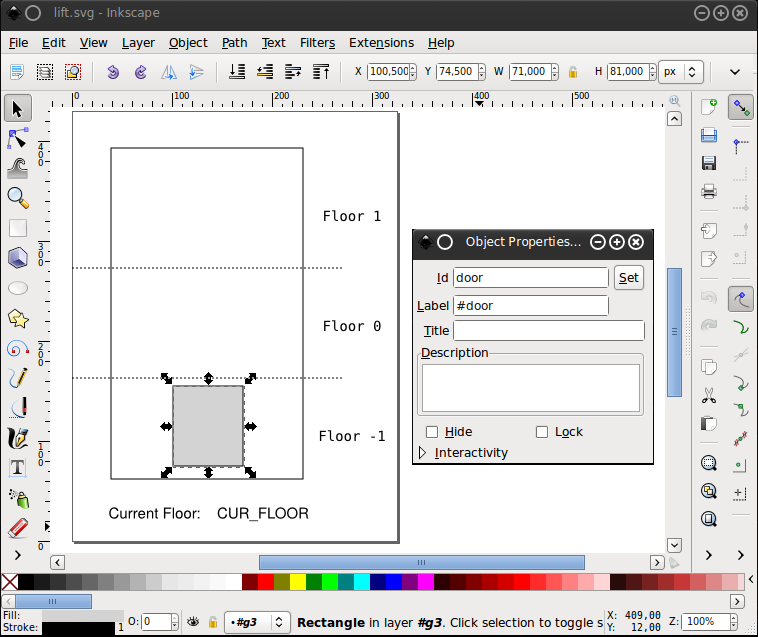
\includegraphics[width=12cm]{img/tutorial/tut_02.png}
	\caption{Creating an SVG graphic with Inkscape}
	\label{fig_tut_02_inkscape}
\end{center}
\end{figure} 

\paragraph{\texttt{bmotion.vis.js and require.js:}}
These JavaScript libraries are needed to run the visualization.
Do not edit them!

\section{Link a Model with the Visualisation}

In order to link a model with a visualization, open the \texttt{bmotion.json} file with an editor of your choice and set the \textit{model} path (e.g. ``model/my-model.mch''):
Linking a model within \texttt{bmotion.json} file automatically loads the model, when starting the visualisation.

To create a link between graphical elements and the model, please checkout the Section about observers (\ref{tutorial_b} for Event-B and Classical-B or \ref{tutorial_csp} for CSP).
